\documentclass[a4paper]{report}
\author{Jure Kos}
\title{Vaja 68, Fotoefekt}
\date{3.3.2022}
\usepackage{graphicx}
\graphicspath{ {./images/} }

\begin{document}

\maketitle

\chapter*{Uvod}
Fotoefekt je pojav, pri katerem obsevanje z elektromagnetnim valovanjem
povzroča izletavanje elektronov iz površine kovine. Energija izstopajočih
elektronov je sorazmerna frekvenci in neodvisna od intenzitete svetlobnega
toka. Klasično pojmovanje svetlobe kot valovanja pojava ne pojasnjuje,
zato moramo privzeti, da se svetloba obnaša, kot da bi jo sestavljali delci -
fotoni. Fotoelektrični pojav lahko sedaj pojasnimo s tem, da so elektroni v
kovini vezani, kar pomeni, da jo zapustijo samo, če jim dovedemo energijo
večjo ali enako vezavni energiji. Elektron pri tem opravi izstopno delo
$A_i$. Energija fotona $h\ni$, ki povzroči izlet elektrona mora biti torej večja ali enaka
izstopnemu delu, energija elektrona pa je enaka:

\[W_k = h\nu - A_i\]

Kjer je $\nu$ frekvenca vpadnega valovanja, h pa Planckova konstanta.

Pojav opazujemo z napravo, ki ji rečemo fotocelica. Slika 1 prikazuje merilno
vezje s fotocelico. Tok skozi fotocelico lahko merimo z občutljivim merilni-
kom električnega toka - galvanometrom. Ko katodo osvetlimo steče tok, ki narašča z intenziteto svetlobe. Elektroni s kinetično energijo $W_k$ dosežejo
anodo, tudi če je med njo in katodo majhna zaporna napetost. Preneha
šele, ko negativna napetost doseže vrednost $U_m$, ki zadrži tudi elektrone z
največjo kinetično energijo. Tedaj velja enačba (2):

\[eU_m = W_e = h\nu - A_i\]

Iz diagrama tok - napetost lahko določimo maksimalno negativno napetost
$U_m$ v točki, ko preneha teči tok. Z osvetljevanjem fotocelice s svetlobo
različnih valovnih dolžin določimo ustrezne energije izstopajočih elektro-
nov, v diagramu energija elektronov - frekvenca svetlobe iz naklona premice
določimo Planckovo konstanto
h, iz njenega premika vzdolž osi energije pa
ocenimo izstopno delo $A_i$

\chapter*{Naloga}
Preveri linearno zvezo med frekvenco svetlobe
$\nu$
in energijo fotona. Določi
Planckovo konstanto in izstopno delo!

\section*{Potrebščine}

1. Optična klop,\\
2. živosrebrna luč s transformatorjem,\\
3. zaslonka,\\
4. filtri za svetlobo,\\
5. fotocelica z vezalno ploščo,\\
6. izvor napetosti,\\
7. ampermeter.


\chapter*{Meritve}


\noindent $\lambda$ = 365nm \\
\begin{center}
\begin{tabular}{ |c|c| } 
 \hline
 I [A] $\pm 0.005$ [A] & U [V] $\pm 0.001$\\
 \hline
    18    & -0,50 \\
    15    & -0,60 \\
    13    & -0,80 \\
    11    & -0,90 \\
    9     & -1,00 \\
    7     & -1,10 \\
    5     & -1,25 \\
    3     & -1,35 \\
    1     & -1,50 \\
    1     & -1,59 \\
    0     & -1,60 \\
    0     & -1,65 \\
 
\hline
\end{tabular}
\end{center}


\noindent $\lambda$ = 405nm \\
\begin{center}
\begin{tabular}{ |c|c| } 
 \hline
 I [A] $\pm 0.005$ [A] & U [V] $\pm 0.001$\\
 \hline
    10    & -0,75 \\
    5     & -0,95 \\
    3     & -1,05 \\
    2     & -1,10 \\
    1     & -1,15 \\
    1     & -1,20 \\
    1     & -1,22 \\
    0,5   & -1,25 \\
    0,5   & -1,27 \\
    0     & -1,28 \\
    0     & -1,30 \\
\hline

\end{tabular}
\end{center}

\newpage

\noindent $\lambda$ = 436nm \\
\begin{center}
\begin{tabular}{ |c|c| } 
 \hline
 I [A] $\pm 0.005$ [A] & U [V] $\pm 0.001$\\
 \hline
    10    & -0,75 \\
    5     & -0,90 \\
    3     & -1,00 \\
    2     & -1,04 \\
    1     & -1,06 \\
    0,5   & -1,09 \\
    0,5   & -1,10 \\
    0     & -1,11 \\
\hline

\end{tabular}
\end{center}


\noindent $\lambda$ = 546nm \\
\begin{center}
\begin{tabular}{ |c|c| } 
 \hline
 I [A] $\pm 0.005$ [A] & U [V] $\pm 0.001$\\
 \hline
    10    & -0,40 \\
    5     & -0,43 \\
    3     & -0,50 \\
    2     & -0,53 \\
    1     & -0,57 \\
    0,5   & -0,60 \\
    0,5   & -0,61 \\
    0     & -0,62 \\
\hline

\end{tabular}
\end{center}


\noindent $\lambda$ = 577nm \\
\begin{center}
\begin{tabular}{ |c|c| } 
 \hline
 I [A] $\pm 0.005$ [A] & U [V] $\pm 0.001$\\
 \hline
    10    & -0,10 \\
    5     & -0,25 \\
    3     & -0,30 \\
    2     & -0,35 \\
    1     & -0,40 \\
    1     & -0,42 \\
    0,5   & -0,43 \\
    0     & -0,44 \\
\hline

\end{tabular}
\end{center}



\chapter*{Grafi}

\begin{figure}[htp]
    \centering
    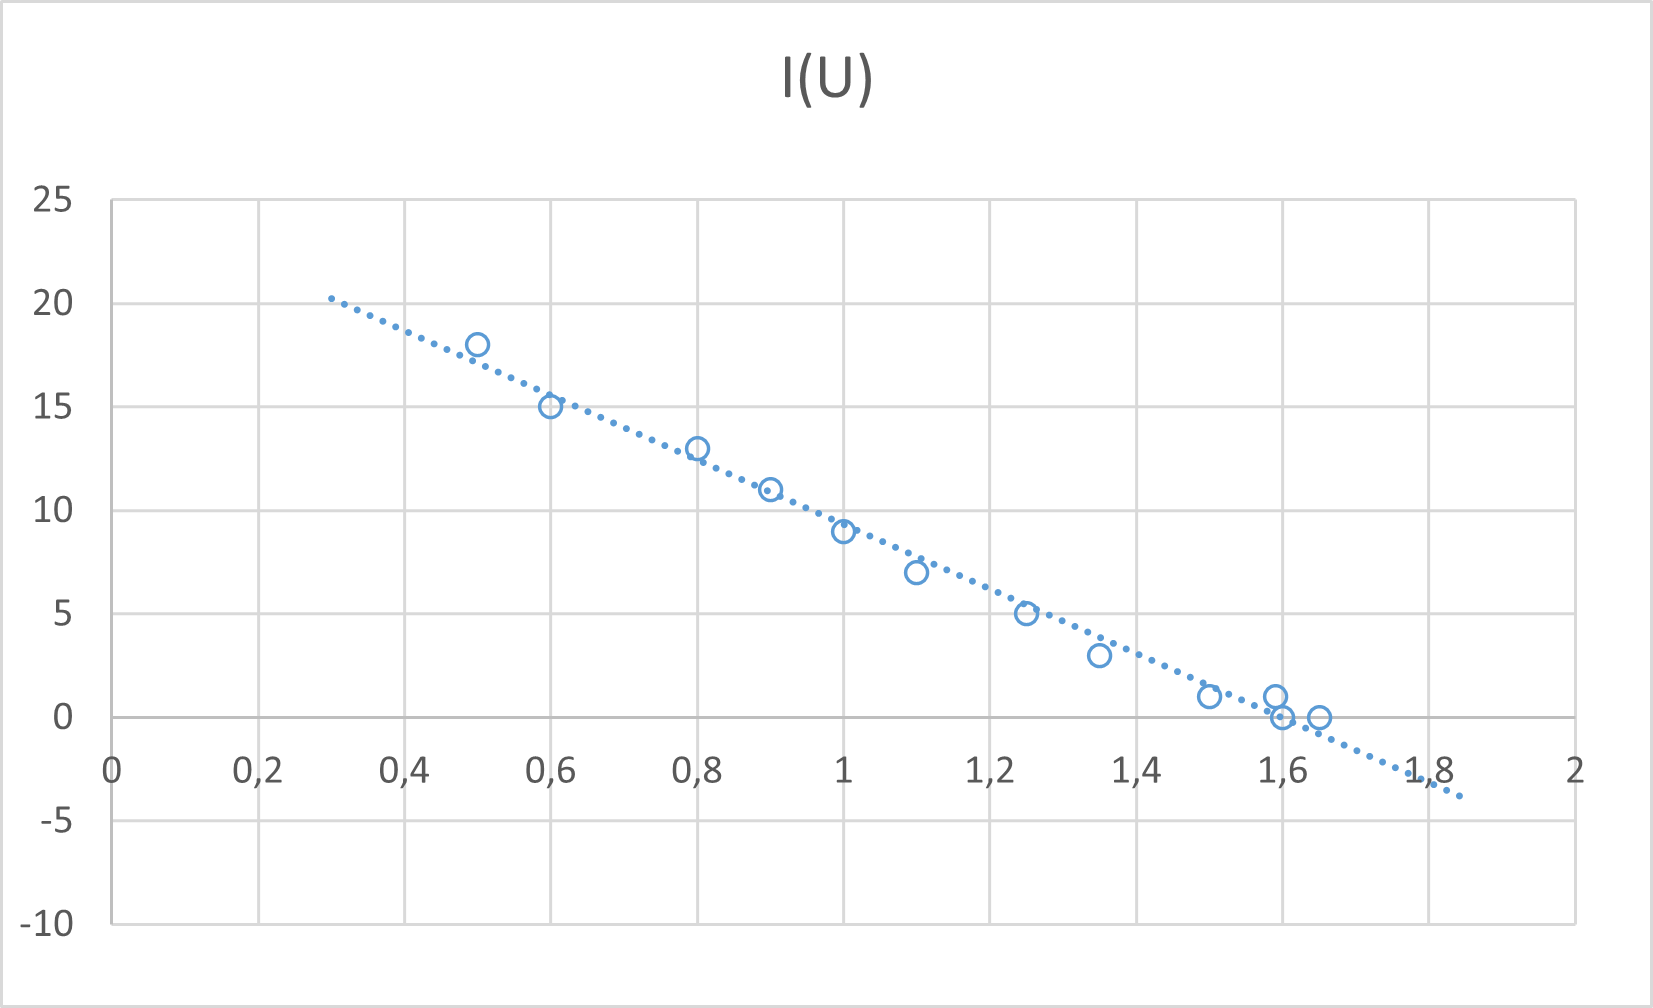
\includegraphics[width=\textwidth]{energija in frekvenca graf 1.png}
    \caption{365nm graf}
    
\end{figure}

\begin{figure}[htp]
    \centering
    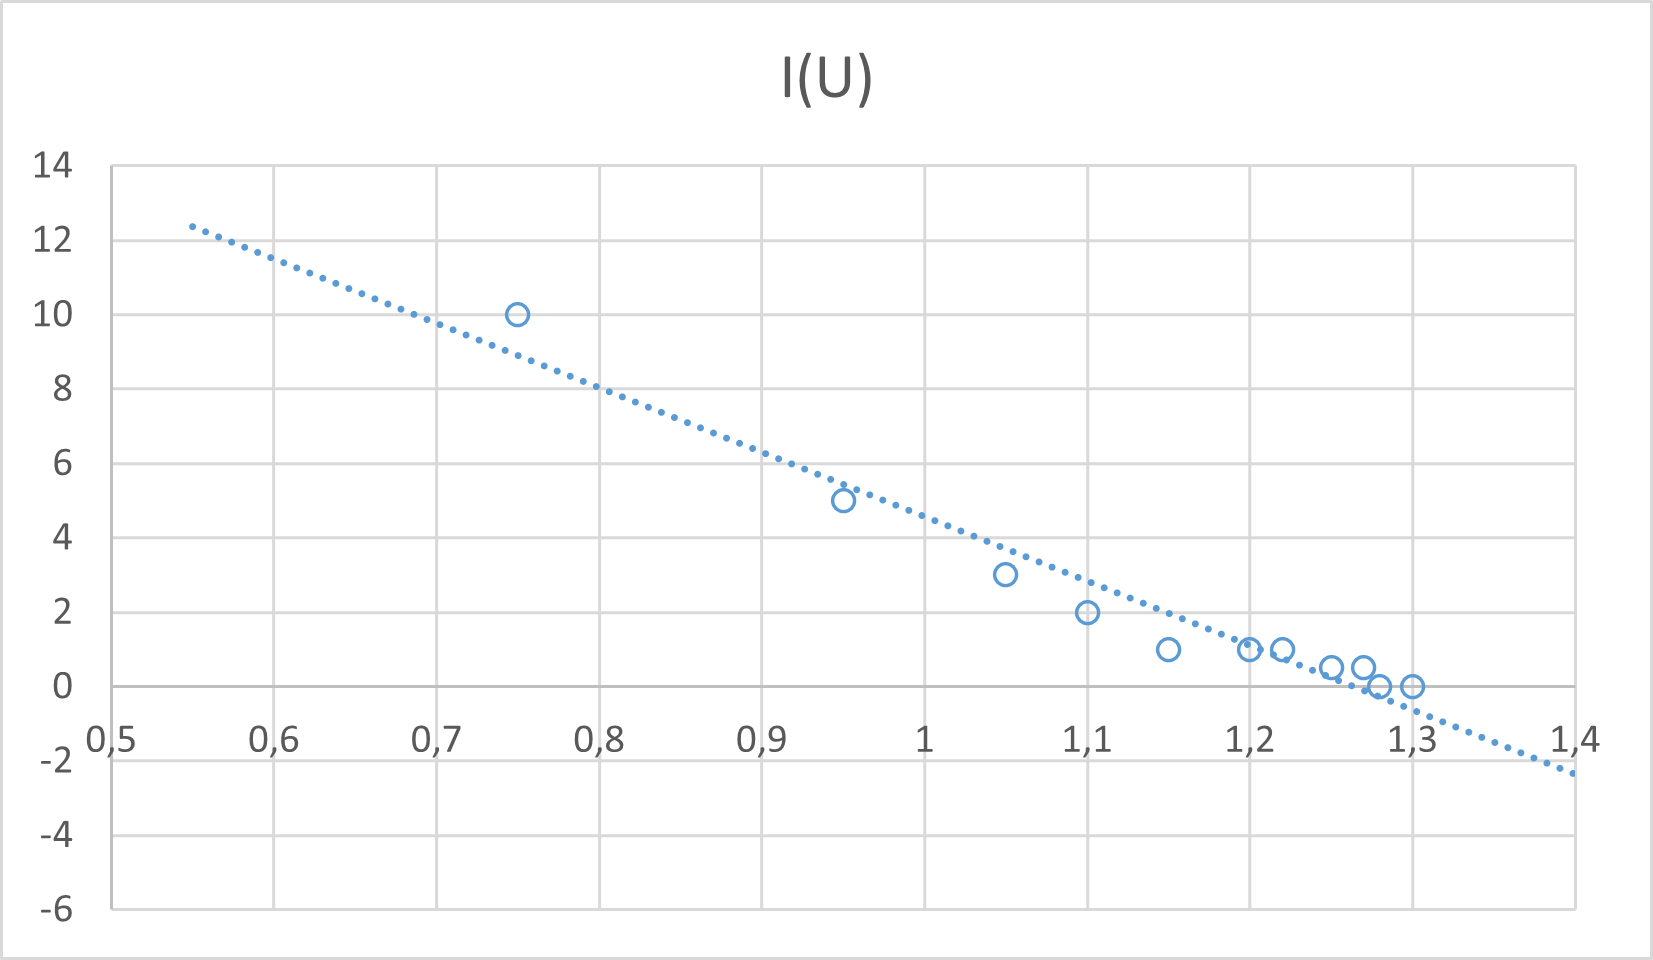
\includegraphics[width=\textwidth]{energija in frekvenca graf 2.png}
    \caption{405nm graf}

\end{figure}

\begin{figure}[htp]
    \centering
    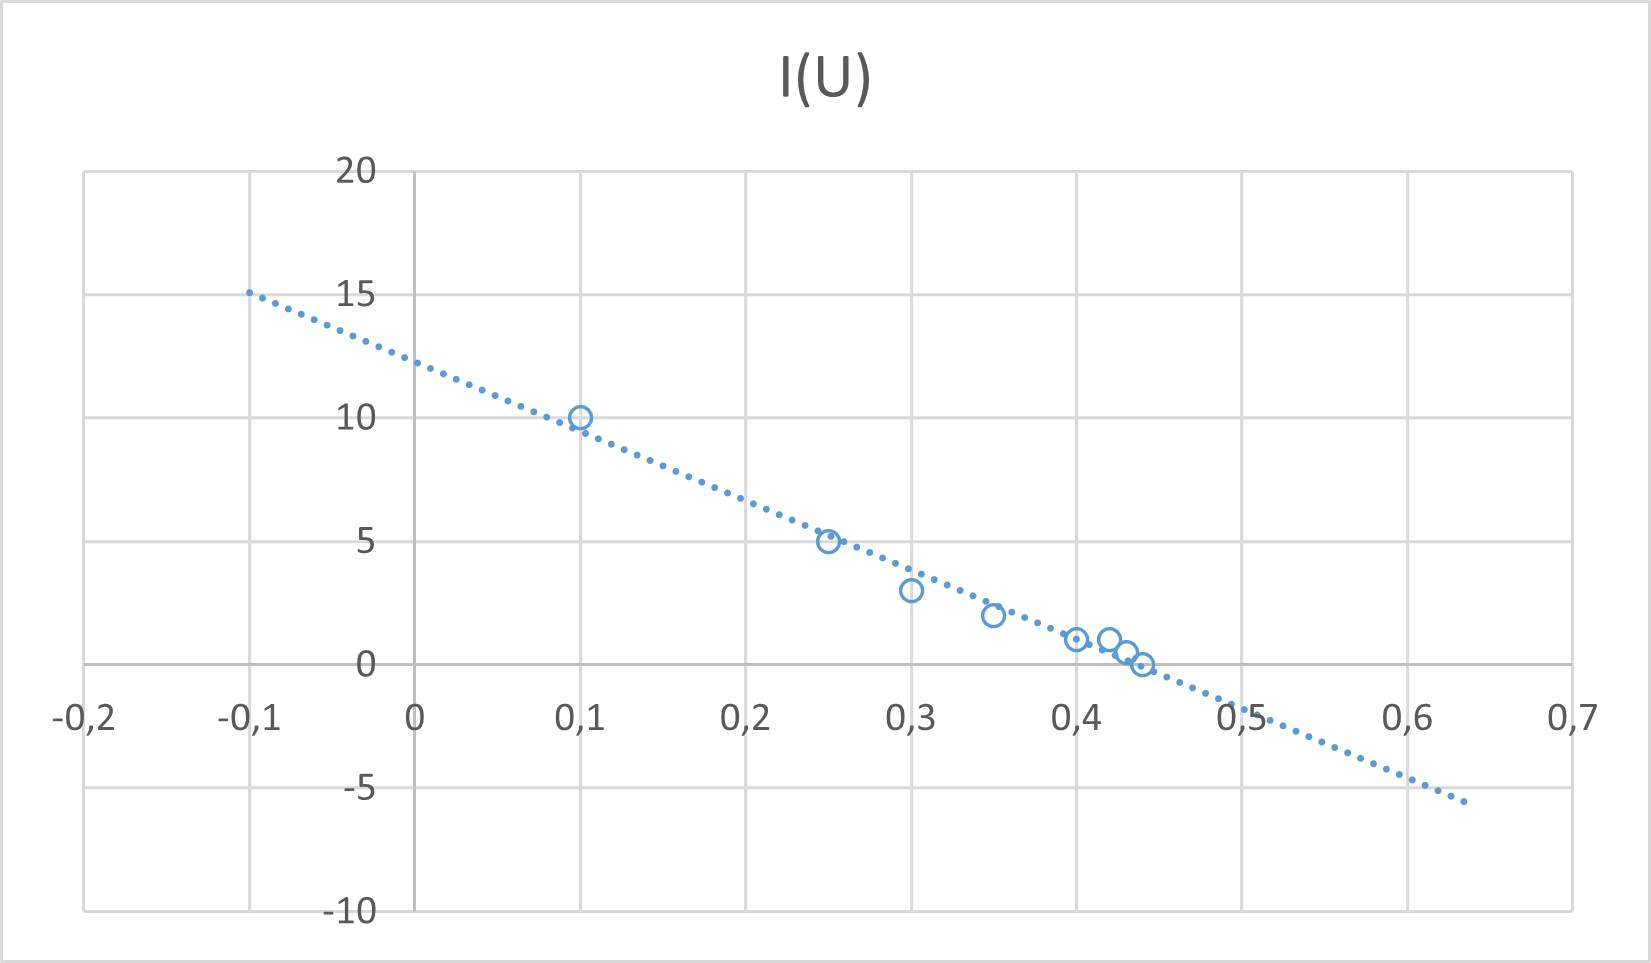
\includegraphics[width=\textwidth]{energija in frekvenca graf 3.png}
    \caption{436nm graf}

\end{figure}

\begin{figure}[htp]
    \centering
    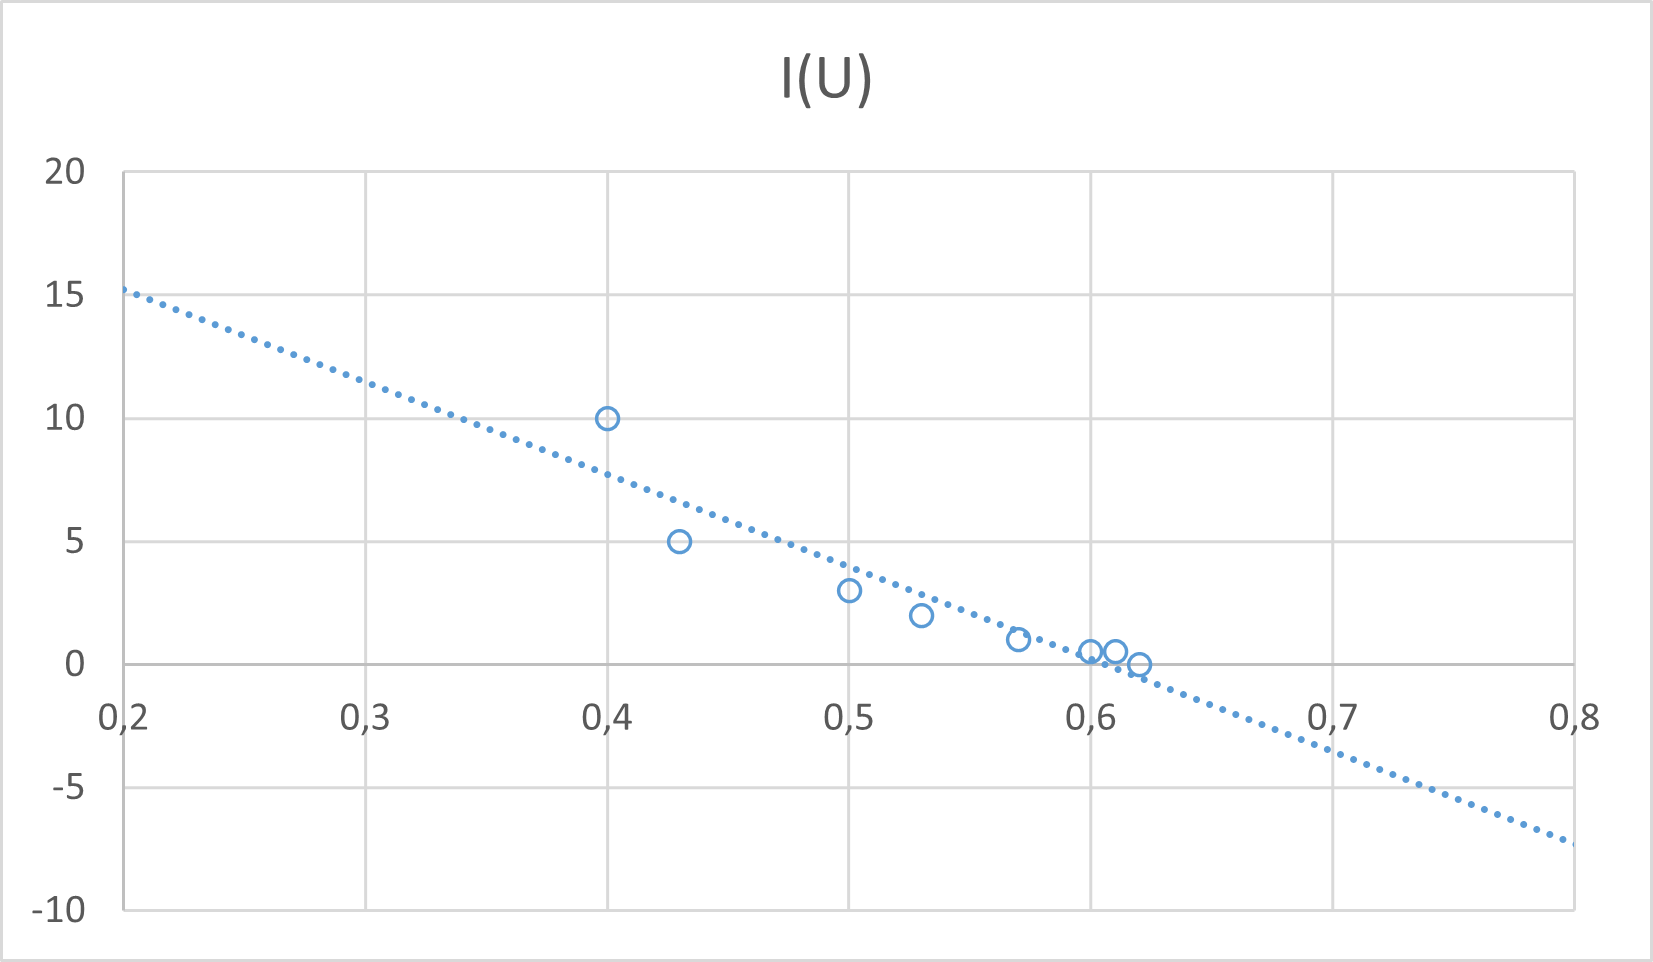
\includegraphics[width=\textwidth]{energija in frekvenca graf 4.png}
    \caption{546nm graf}

\end{figure}

\begin{figure}[htp]
    \centering
    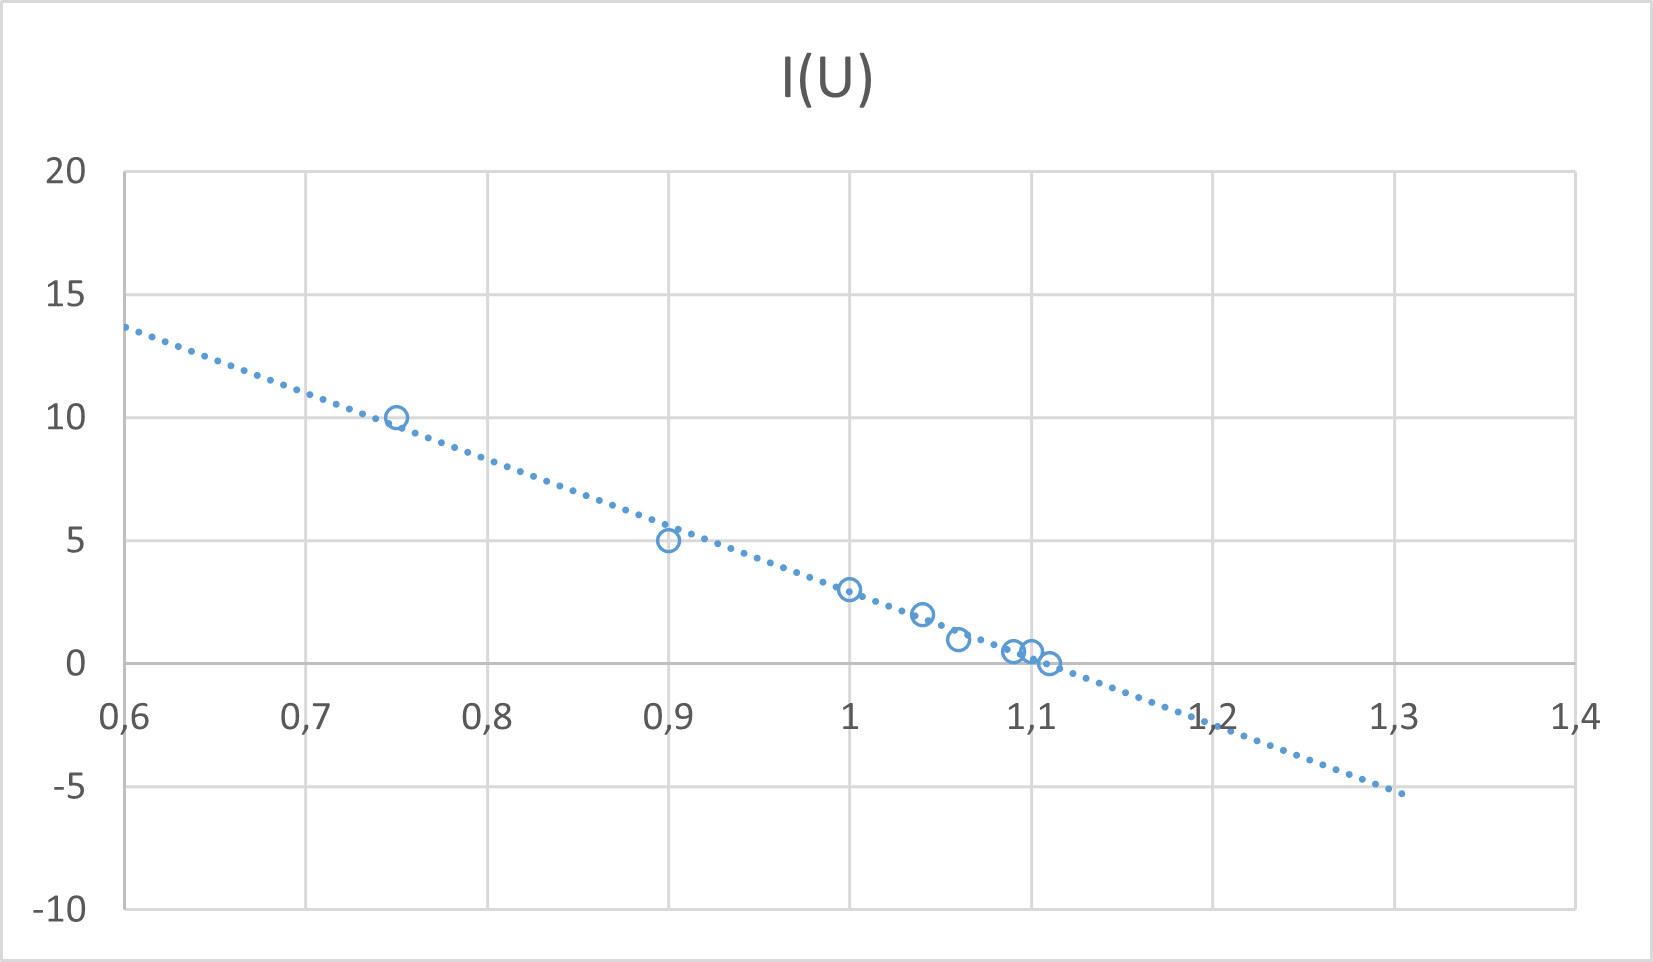
\includegraphics[width=\textwidth]{energija in frekvenca graf 5.png}
    \caption{577nm graf}

\end{figure}

\chapter*{Računi}
Za določitev Planckove konstante, za vsako valovno dolžino izberemo napetost $U_m$ pri kateri tok več ne raste:
\\
\begin{center}
\begin{tabular}{ |c|c| }
 \hline
 365nm & -1.60V \\
 405nm & -1.26V \\
 436nm & -1.11V \\
 546nm & -0.60V \\
 577nm & -0.44V  \\
 \hline
\end{tabular}
\end{center}

\noindent Tedaj velja 
\[W_k = U_m \cdot e = h\nu - A_i\]


\begin{figure}[htp]
    \centering
    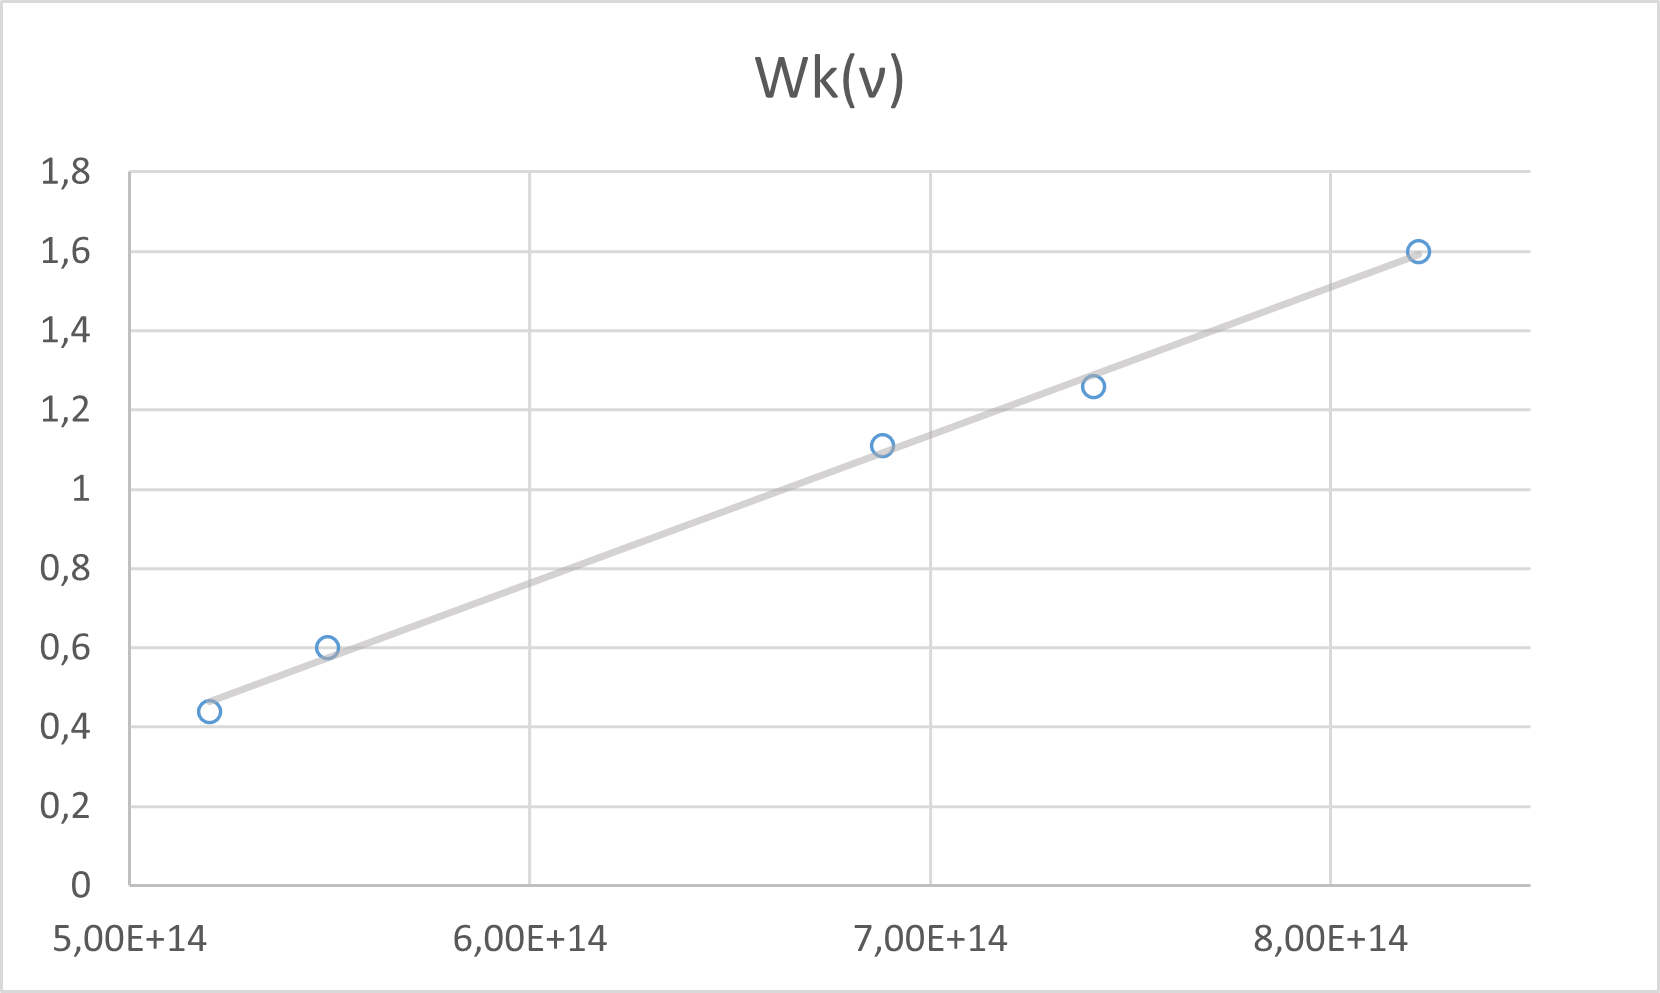
\includegraphics[width=15cm]{energija in frekvenca graf.png}
    \caption{graf prikazuje odvisnost  zaporne napetosti od  frekvence $\nu$ svetlobe}
    \label{fig:galaxy}
\end{figure}

\newpage

Premica, ki se najbolje prilega meritvam ima enačbo 

\[W_k =k\nu -n= h\nu - A_i\] 

kjer je $k = 3,74 \cdot 10^-{15}eVs$ ter $n = -1,48 eV$.\\\\
Iz tega sledi

\[h = 3,74 \cdot 10^{-15} eVs \pm0.4 \cdot 10^{-15} eVs\]

in

\[A_i = 1,48 eV \]

\end{document}
